\documentclass[english]{article}
\usepackage[T1]{fontenc}
%\usepackage[latin9]{inputenc}
\usepackage[utf8]{inputenc}
\usepackage{float}
\usepackage{caratula}
\usepackage{graphicx}
\usepackage{babel}


% Variables de Titulo
\universidad{Instituto Tecnológico de Buenos Aires}
\facultad{Ingeniería Informática}
\departamento{Sistemas Operativos}
\materia{Trabajo Práctico 2}
\titulo{Multitasker}
\integrante{Castiglione, Gonzalo}{Legajo: 49138}
\integrante{Gomez, Horacio}{Legajo: 50825}
\integrante{Orsay, Juan Pablo}{Legajo: 49373}
\fecha{Segundo cuatrimestre de 2011}
\footspace{3cm}

% Otras Variables
\newtheorem{hip}{Hipótesis}

% Headers & Footers
\usepackage{fancyhdr}
\setlength{\headheight}{15pt} 
\pagestyle{fancy}

\fancyhead{} % Clear all header fields
\fancyhead[RE,LO]{Trabajo Práctico 2 - 2do Cuatrimestre 2011}
\fancyhead[LE,RO]{
\includegraphics[height=13pt]{logop.jpg}}
\fancyfoot{} % Clear all footer fields
\fancyfoot[LE,RO]{\thepage\ de \pageref{LastPage}}

\begin{document}

\maketitle
\newpage

% Generar el indice
\setcounter{page}{1} %Resetea el contador para que no cuente la hoja del titulo.
\tableofcontents
\newpage

\section{Procesos}

Para implementar procesos inicialmente se decidió utilizar como base el código proveído por la cátedra. Luego de bastante tiempo sin llegar a nada, se decidió comenzar desde cero.

Se realizó un diagrama del stack necesario para un proceso resultando en el siguiente:

\begin{figure}[H]
\begin{center}
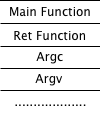
\includegraphics[width=5cm,height=2.5cm,keepaspectratio]{stack}

\caption{Stack frame}
\end{center}
\end{figure}

Una vez realizado ése diagrama, se procedió a armar manualmente el stack para correr el sistema operativo, haciendo que la función kmain sea solo una función dummy que llamase a una función de assembler para que crease dicho stack frame. Una vez construido éste, se cambió el ESP con otra función de assembler y el sistema siguió ejecutando en la función indicada por el stack frame.

Luego de entender como funciona el stack para ejecutar una función determinada, pasandole ciertos argumentos y haciendo que en su retorno, vaya a otra función, se procedió a crear una función que agregase éstos "procesos" a una lista para que luego puedan ser procesados por el scheduler.

\subsection{Scheduler}
Se decidió implementar un scheduler con prioridad, y un scheduler de tipo Round Robin.
Éste inicialmente se disparaba cada dos ticks, pero eso hacía el sistema muy lento.

\subsubsection{Scheduler con prioridad}
Al usar un scheduler con prioridad, los procesos pasan a ser más o menos importantes dependiendo de que prioridad se le asignó en su creación. Los procesos lanzados por el usuario mediante comandos en la consola son creados con una determinada prioridad. Hay un grupo de procesos que corre con prioridades especiales, uno de ellos el el proceso \emph{idle}.

Éste corre con prioridad muy baja, dado que es el que se ejecuta cuando no hay ningún otro proceso listo para ejecutarse. Otro grupo de procesos que corre con prioridad especial son las shells.

Las shells no son bloqueantes, por lo que constantemente están polleando el tecleado para ver si hay nuevos caracteres que mostrar. Esto hace que sea necesario que éstas tengan distintas prioridades dependiendo de si están activas o no. La activa pasa a tener más de un 80\% del uso del procesador, y las restantes menos de un 5\%. Al cambiar, se actualizan las prioridades de éstas (esto es posible ya que las prioridades de los procesos son dinámicas, y, si bien no se presenta ningún comando para cambiarlas, se pueden cambiar)

\subsection{Estados}
Cada proceso puede tener alguno de los siguientes estados:
\begin{itemize}
\item READY: El proceso está listo para ejecutarse
\item RUNNING: El proceso está siendo ejecutado en ese momento
\item CHILD\_WAIT: El proceso está bloqueado esperando que algún hijo finalice. Esto sucede cuando, por ejemplo, una consola ejecuta un proceso en \emph{foreground}.
\end{itemize}

\pagebreak{}

\section{Driver disco ATA}

La implementación de driver \emph{ATA} que se utilizó en este Sistema Operativo permite
acceso a un sector con offset y tamaño arbitrario (tanto para lectura
como para escritura). Si bien realizar esto dificultó la programación
del driver, permite tener una lógica de programación más simple en
las capas superiores ya que no es necesario leer un sector entero
para luego ir hasta el offset deseado y obtener de ahí los bytes
necesarios (ni hablar si se quiere tomar información que se encuentra
partida en varios sectores contiguos). Es por eso que el driver utilizado
permite \emph{abstraerse} de esta división por sectores y poder acceder
a disco a partir de un sector con cualquier offset y cualquier cantidad
de bytes que se quiera leer.

La implementación utilizada además presenta métodos para detección
de las propiedades de un disco (Si es removible, ATA, soporta DMA
y LBA), no se pudo (por falta de tiempo) crear un comando para listar
las cualidades de los discos conectados desde las consolas, pero se
espera poder mostrarlos para la próxima entrega.

Un detalle a mencionar es que la escritura al disco con un offset
es muy cara ya que ATA solo permite escribir de un sector entero,
por lo que para escribir una parte de uno de estos, primero hay que
leerlo entero en un buffer auxiliar, luego pisar los lugares a cambiar
y luego guardarlos, lo que seria equivalente a dos accesos a disco
solo para grabar una $x$ cantidad de bytes. Por lo que siempre se
intentará grabar la mayor cantidad de bytes posibles en cada acceso.

\pagebreak{}


\section{Disk Cache}

Debido a los problemas de eficiencia mencionados en la sección anterior,
se decidió que seria una buena idea tener una estructura cache, que
minimize los accesos a discos sin consumir mucha cantidad de memoria
ni procesamiento. 

La implementación de esta capa consiste en un vector de $N$ estructuras 
en la que cada una tiene el contenido de un sector entero de disco y campos 
para indicar si el sector se encuentra sucio (si tiene cambios con respecto 
al disco) y a que sector y disco corresponde.

El algoritmo de reemplazo elegido es el de LRU (el que menos accesos
tuvo, se reemplaza). 

Un problema al implementar esta capa fue decidir que hacer con los sectores
sucios ya que como se encuentran en RAM, hasta no ser guardados, la
información es propensa a perderse (ya sea por fallas del sistema,
corte de luz, etc). Frente a esto se decidió que cada una cantidad
fija de $ticks$, todos los sectores sucios serían escritos a disco. 

\pagebreak{}


\section{File System}

Este File System se divide en dos partes, la primer parte es, el
file system en si y la segunda es la administración de la infomación
en el disco ($DiskManager$).

Para el manejo de archivos se decidió tomar la misma implementación
que usa Linux. Es decir, archivos regulares, directorios, symbolic
links, etc son todos la misma estructura $fs$\_$node$ y lo único
que los diferencía es su campo $mask$ (en donde se define el tipo).
Inicialmente se comenzó tratando a cada tipo de archivo como un tipo
de estructura diferente, pero terminamos concluyendo que se volvía
muy compleja la lógica de parseo de información en el disco.


\subsection{Manejo de disco}

Debido a la notable lentitud que posee el acceso a disco frente el
acceso a RAM, se diseñó el almacenamiento de la información dando
mas importancia siempre a la cantidad de accesos a disco por sobre
cantidad de bytes desperdiciados por archivo.

Uno de los primeros problemas que se presentaron al comenzar a trabajar
en disco, era como averiguar si un determinado sector de memoria era
o no válido. Frente a esto, en cada Header (mas adelante se hablará
mejor de estos) se agregó un campo $magic$ que sirve para la validación
de los campos a leer. En otras palabras, si el magic number del header
leído coincide con el magic number definido en el SO, entonces existe
una estructura válida almacenada en esa posición de memoria. \\


El disco duro para este file system fue dividido básicamente en cuatro
partes:
\begin{enumerate}
\item File System header
\item Memory bitmap (bloques libres y ocupados en el disco)
\item Vector de iNodos
\item Archivos
\end{enumerate}

\begin{figure}[H]
\begin{center}
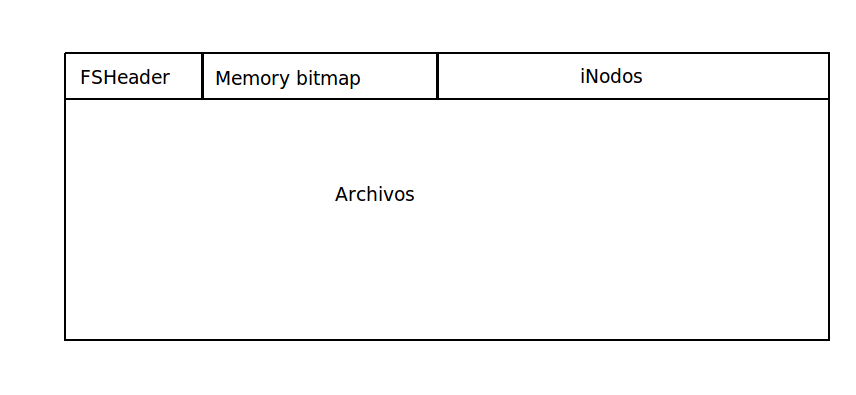
\includegraphics[width=10cm,height=5cm,keepaspectratio]{Imagen_disco}

\caption{Imagen disco duro}
\end{center}
\end{figure}


Para el F.S. Header simplemente se guardó un magic number y dos números
mas para indicar el tamaño máximo del vector de inodos y la cantidad
actual de inodos que se tienen guardados.

Cuando el S.O. se inicializa, intenta leer este sector de memoria, si
el magic number es válido, quiere decir que existe una partición valida
y entonces se intenta cargarla.

En cuanto al vector de iNodos, se trata de un vector de $N$ estructuras
de tamaño fijo (muy importante!) ya que permite el acceso al elemento
$i$ mediante una simple operación matemática. En cada posición del vector, 
se tiene almacenada una estructura de tipo $DiskPage$, para indicar en que 
bloque del disco puede la información ser encontrada y dos enteros: uno para 
indicar la cantidad de bloques que esta página tiene reservada para su uso y 
otro para la cantidad de bytes utilizados por el contenido del usuario.

La parte del disco dedicada a archivos se encuentra dividida en bloques
de tamaño fijo definido por el SO. Lo mas importante para destacar
en esta parte es la forma que se tiene para el almacenamiento de cada
archivo, el formato elegido para el almacenamiento de la información
es muy parecido al de una $LinkedList$. Todo archivo en disco consiste
de:
\begin{enumerate}
\item Disk Page
\item File Header
\item Su contenido
\end{enumerate}

\begin{figure}[H]
\begin{center}
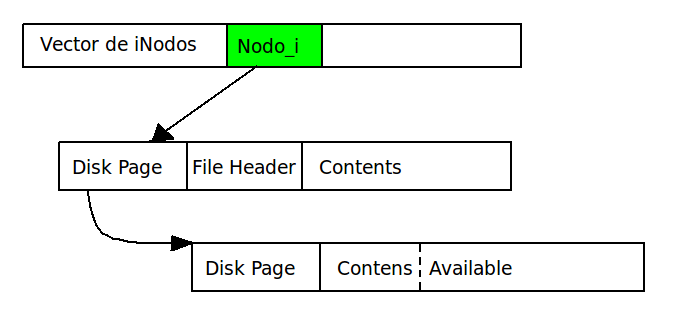
\includegraphics[width=10cm,height=7cm,keepaspectratio]{Archivo}

\caption{Formato de almacenamiento de un archivo}
\end{center}
\end{figure}


La estructura $File$$Header$ se guarda una única vez por cada archivo
y es la que posee el nombre, tipo, permisos y demás atributos que
no son parte del contenido en si.\\


El primer algoritmo que se utilizó para reservar memoria para un archivo
consistía en ir leyendo cada bloque del disco desde el principio
y marcar los headers de los bloques que necesitasen y esten disponibles. 
Inicialmente parecía funcionar bien (ya que no se trabajaba con mas de 2 o 3
 archivos en total), pero, a medida que se requería de mayor cantidad de 
archivos y carpetas, nos dimos cuenta de lo terriblemente
lento que se volvía este algoritmo. Luego se lo reemplazó por uno
que utiliza un $memory$ $bitmap$, el cual se encuentra junto al
FS header completando todo el primer sector del disco. Cada bit de este
mapa, indica si el bloque $i$ de la parte de archivos se encuentra
ocupada o libre. De esta manera, consultar si un bloque se encuentra disponible 
requiere ahora moverse sobre un arreglo de bits cargado en RAM en vez de 
sectores en disco! Y los únicos accesos son para escribir los headers de las 
páginas a utilizar.


\subsection{Manejo en RAM}

El manejo de inodos es ram es bastante sencillo, el $F.S.$ mantiene
un vector con los últimos inodos consultados y ofrece la interfaz
para el SO para la modificiación y consulta de estos úlimos en disco.
Cada vez que un nuevo inodo es consultado, se toma la siguiente posición
del vector y se carga allí la información de disco de este inodo para
luego retornarla.

Un detalle a tener en sobre esta implementación de $F.S.$, es que
no guarda ningún contenido de archivos (no cachea), ya que consideramos
que eso debe ser trabajo de una capa mas entre el $diskManager$ y
el driver de disco ($diskCache$).

\pagebreak{}

\section{Permisos}

\subsection{Alta-Baja-Modificación de Usuarios.}
El sistema posee de un array de usuarios que es cargado en el startup llamando a la función $user_init()$, el mismo se mantiene en memoria a lo largo de toda la ejecución del sistema. Inspirados en la implementación de Linux, los usuarios son parseados de un archivo localizado en /etc/passwd que contiene en cada línea un string de estas características:
$$uid:gid:username:password$$
Cada vez que se realiza un cambio en el array de usuarios, se llama a la función de flush para actualizar el archivo correspondiente con los cambios.
Las siguientes son las system-calls que se pueden utilizar para el manejo de usuarios:
\begin{itemize}

\item $userlist$: lista los usuarios del sistema.
\subitem Cualquier usuario puede utilizar este comando.

\item $useradd USERNAME PASSWORD$: agrega un nuevo usuario al sistema.
\subitem Cualquier usuario puede utilizar este comando.
\subitem El usuario se crea dentro del grupo del usuario logueado.

\item $userdel USERNAME$: borra el usuario del sistema.
\subitem Sólo root o el dueño del grupo al que pertenecen puede borrar usuarios.
\subitem No se puede borrar el usuario logueado.

\end{itemize}
 
\subsection{Alta-Baja-Modificación de Grupos.}
Análogo al sistema de usuarios con la salvedad de que el archivo de persistencia es /etc/group y los strings tienen la siguiente forma:
$$gid:groupname:password$$
Las siguientes son las system-calls que se pueden utilizar para el manejo de grupos:
\begin{itemize}

\item \emph{grouplist}: lista los grupos del sistema.
\subitem Cualquier usuario puede utilizar este comando.

\item \emph{groupadd GROUPNAME PASSWORD}: agrega un nuevo grupo al sistema.
\subitem Cualquier usuario puede utilizar este comando.
\subitem El grupo se crea con gid libre.

\item \emph{groupdel GROUPNAME}: borra el grupo del sistema.
\subitem Sólo root o el dueño puede borrar un grupo.
\subitem No se puede borrar el grupo del usuario logueado.

\end{itemize}

 
\subsection{Accesos}
Una vez que se posee en memoria una base de datos de usuarios y grupos, junto con los datos del usuario que está logueado en la sesión se pueden realizar chequeos de acceso.

\subsection {Permisos de File-System}
Los permisos sobre el filesystem se chequean de manera similar a la que hace linux. Cada archivo tiene el uid de su dueño y el gid del grupo al cual pertenecen.
Cuando se crea un archivo hereda el uid del usuario logueado y su grupo. En caso de que no exista un usuario logueado (por ejemplo cuando se inicia el sistema) se supone el sistema está en “modo kernel” y se crea todo con uid y gid de root. Con respecto a los permisos se crean con una máscara por defecto de 0x644 que explicaremos luego con más detalle.
Los comandos y system-calls que realizan operaciones sobre archivos poseen llamadas a los métodos de permission.h para verificar que tenga acceso a lo que desea realizar. Por ejemplo al hacer un LS sobre un directorio se chequea que el usuario actual tenga permiso de LECTURA en el mismo. El permiso de lectura puede ser otorgado o no dependiendo de qué permisos posee el directorio.
Si el usuario no es dueño ni parte del grupo al cual pertenece el archivo se chequean los 3 bits menos significativos 0-1-2 (0x007) de la máscara de permisos que posee el mismo, si el usuario, en cambio, es parte del grupo, los bits 3-4-5 (0x070). Si el usuario es el dueño, los bits 6-7-8 (0x700).
Si el usuario logueado es root, no se chequea ningún permiso, se otorga acceso directamente (esto sirve para por ejemplo modificar archivos que poseen permisos 0x444 o 0x000).
Las siguientes system-calls sólo pueden ser llamadas por el dueño del archivo o root para modificar los permisos del mismo.
\begin{itemize}
\item \emph{chmod OCTAL FILE}: agrega un nuevo grupo al sistema.
\subitem El OCTAL es igual que en Linux ej: 764 = $-rwxrw-r--$
\item \emph{chown USERNAME FILE}: cambia el dueño de un archivo.
\item \emph{chgrp GROUPNAME FILE}: cambia el grupo al que pertenece un archivo.
\end{itemize}
 
\subsection {Permisos en Procesos}
Cuando se crea un proceso, sucede lo mismo que sucede con los archivos, hereda el uid del usuario logueado o root en caso de que no haya uno (“kernel mode”).
Para matar (utilizando el comando kill) un proceso es necesario ser el dueño del mismo o root, en caso contrario se muestra un mensaje de Access denied.
 
\pagebreak{}

\section{Problemas, posibles soluciones y features a agregar}
\begin{itemize}
\item File System
\begin{itemize}
\item Cada vez que se crea un nuevo archivo, el FSHeader es consultado y
se incrementa el valor de la cantidad actual de inodos en el disco
y se utiliza este nuevo valor para utilizar la siguiente posición del
vector de inodos (para el nuevo archivo). Se quiere aclarar que esta
es una implementación que nos parece muy mala y se tiene planeado
cambiarla por una en la que se utilize un bitmap, en donde el bit
$i-esimo$ indicaría si el sector esta libre o no (mismo algoritmo
utilizado para el manejo de espacio de archivos en el disco duro). 
\item Queda a implementar el comando borrar archivo, que esperamos este disponible
para la próxima entrega.
\end{itemize}

\item Pipes
\begin{itemize}
\item No se llegó a terminar el sistema de pipes, por lo que será implementado para el trabajo práctico siguiente.
\end{itemize}

\item Usuarios y Grupos
\begin{itemize}
\item Debido a problemas de último momento, la persistencia de grupos y usuarios se tuvo que inhabilitar. Es decir no se están utilizando los archivos passwd y group, sino que se están levantando una serie de usuarios por defecto que provienen de strings hardcodeados que simulan la lectura de los mencionados archivos. No obstante el sistema de permisos funciona, correctamente. En caso de que se listen archivos donde no existen los usuarios o grupos al cual pertenecen, en la lista figurara como “unknown” en esos campos.
\end{itemize}

\item Memory Management
\begin{itemize}
\item El sistema operativo no cuenta con un manejo adecuado de memoria. No hay posibilidad de liberar los recursos alocados, éste problema será resuelto para la próxima entrega.
\end{itemize}

\item Otros
\begin{itemize}
\item Uno de los problemas mas importantes que tiene la actual versión del
$SO$ es la falta de semáforos y mutexs, especialmente para el momento
de reserva de memoria y para la lectura/escritura de archivos! (problema
de los N lectores y un escritor). Queda en la lista de cosas para
agregar en futuras actualizaciones del SO ya que no pudo ser implementad
por falta de tiempo.
\end{itemize}
\end{itemize}

\end{document}
